{\section{Wyniki pomiarów}}

{\subsection{Cylinder}}

Zaczynając od mniej złożonej bryły. Dla każdego wymiaru dokonanych zostało 5 pomiarów.
Wymiary, które zostały zmierzone, to: średnica zewnętrzna i wewnętrzna cylindra, oraz jego wysokość. \\

Do obliczenia niepewności całkowitej najpierw obliczamy niepewność standardową typu A.
Dla średnicy wewnętrznej niepewność ta wynosi:

\begin{equation*}
    \begin{aligned}
        \displaystyle u_A(x) = \sqrt{ \frac{ \displaystyle \sum_{i=1}^{n} (x_i - \overline{x} )^2 }{ n(n - 1) }  }
        &= \sqrt{ \frac{ (16 - 15.98)^2 + (15.95 - 15.98)^2 + (16 - 15.98)^2 + (16 - 15.98)^2 + (15.95 - 15.98)^2 }{ 5(5 - 1) } } \\
        &= \sqrt{ \frac{ 0.0004 + 0.0009 + 0.0004 + 0.0004 + 0.0009 }{ 20 } }
        = \sqrt{ \frac{ 0.003 }{ 20 } } \approx 0.0122
    \end{aligned}
\end{equation*}

Niepewność standardowa typu B będzie dla każdego wymiaru taka sama,
ponieważ uwzględniamy jedynie błąd przyrządu pomiarowego użytego do każdego pomiaru, którym była suwmiarka o dokładności $0.05mm$.

\begin{equation*}
    \displaystyle u_B(x) = \sqrt{ \frac{ (\Delta_p x)^2 }{3} } = \sqrt{ \frac{ (0.05)^2 }{3} } \approx 0.03
\end{equation*}

Niepewność całkowita będzie równa: 

\begin{equation*}
    u(x) = \sqrt{ u_A^2(x) + u_B^2(x) } = \sqrt{ (0.0122)^2 + (0.03)^2 } \approx 0.32
\end{equation*} 

\newpage

Na wykresach pokazane są pomiary z niepewnością całkowitą (wszędzie równa 0.03) oraz wartością średnią.

\begin{figure}[ht]
    \centering
    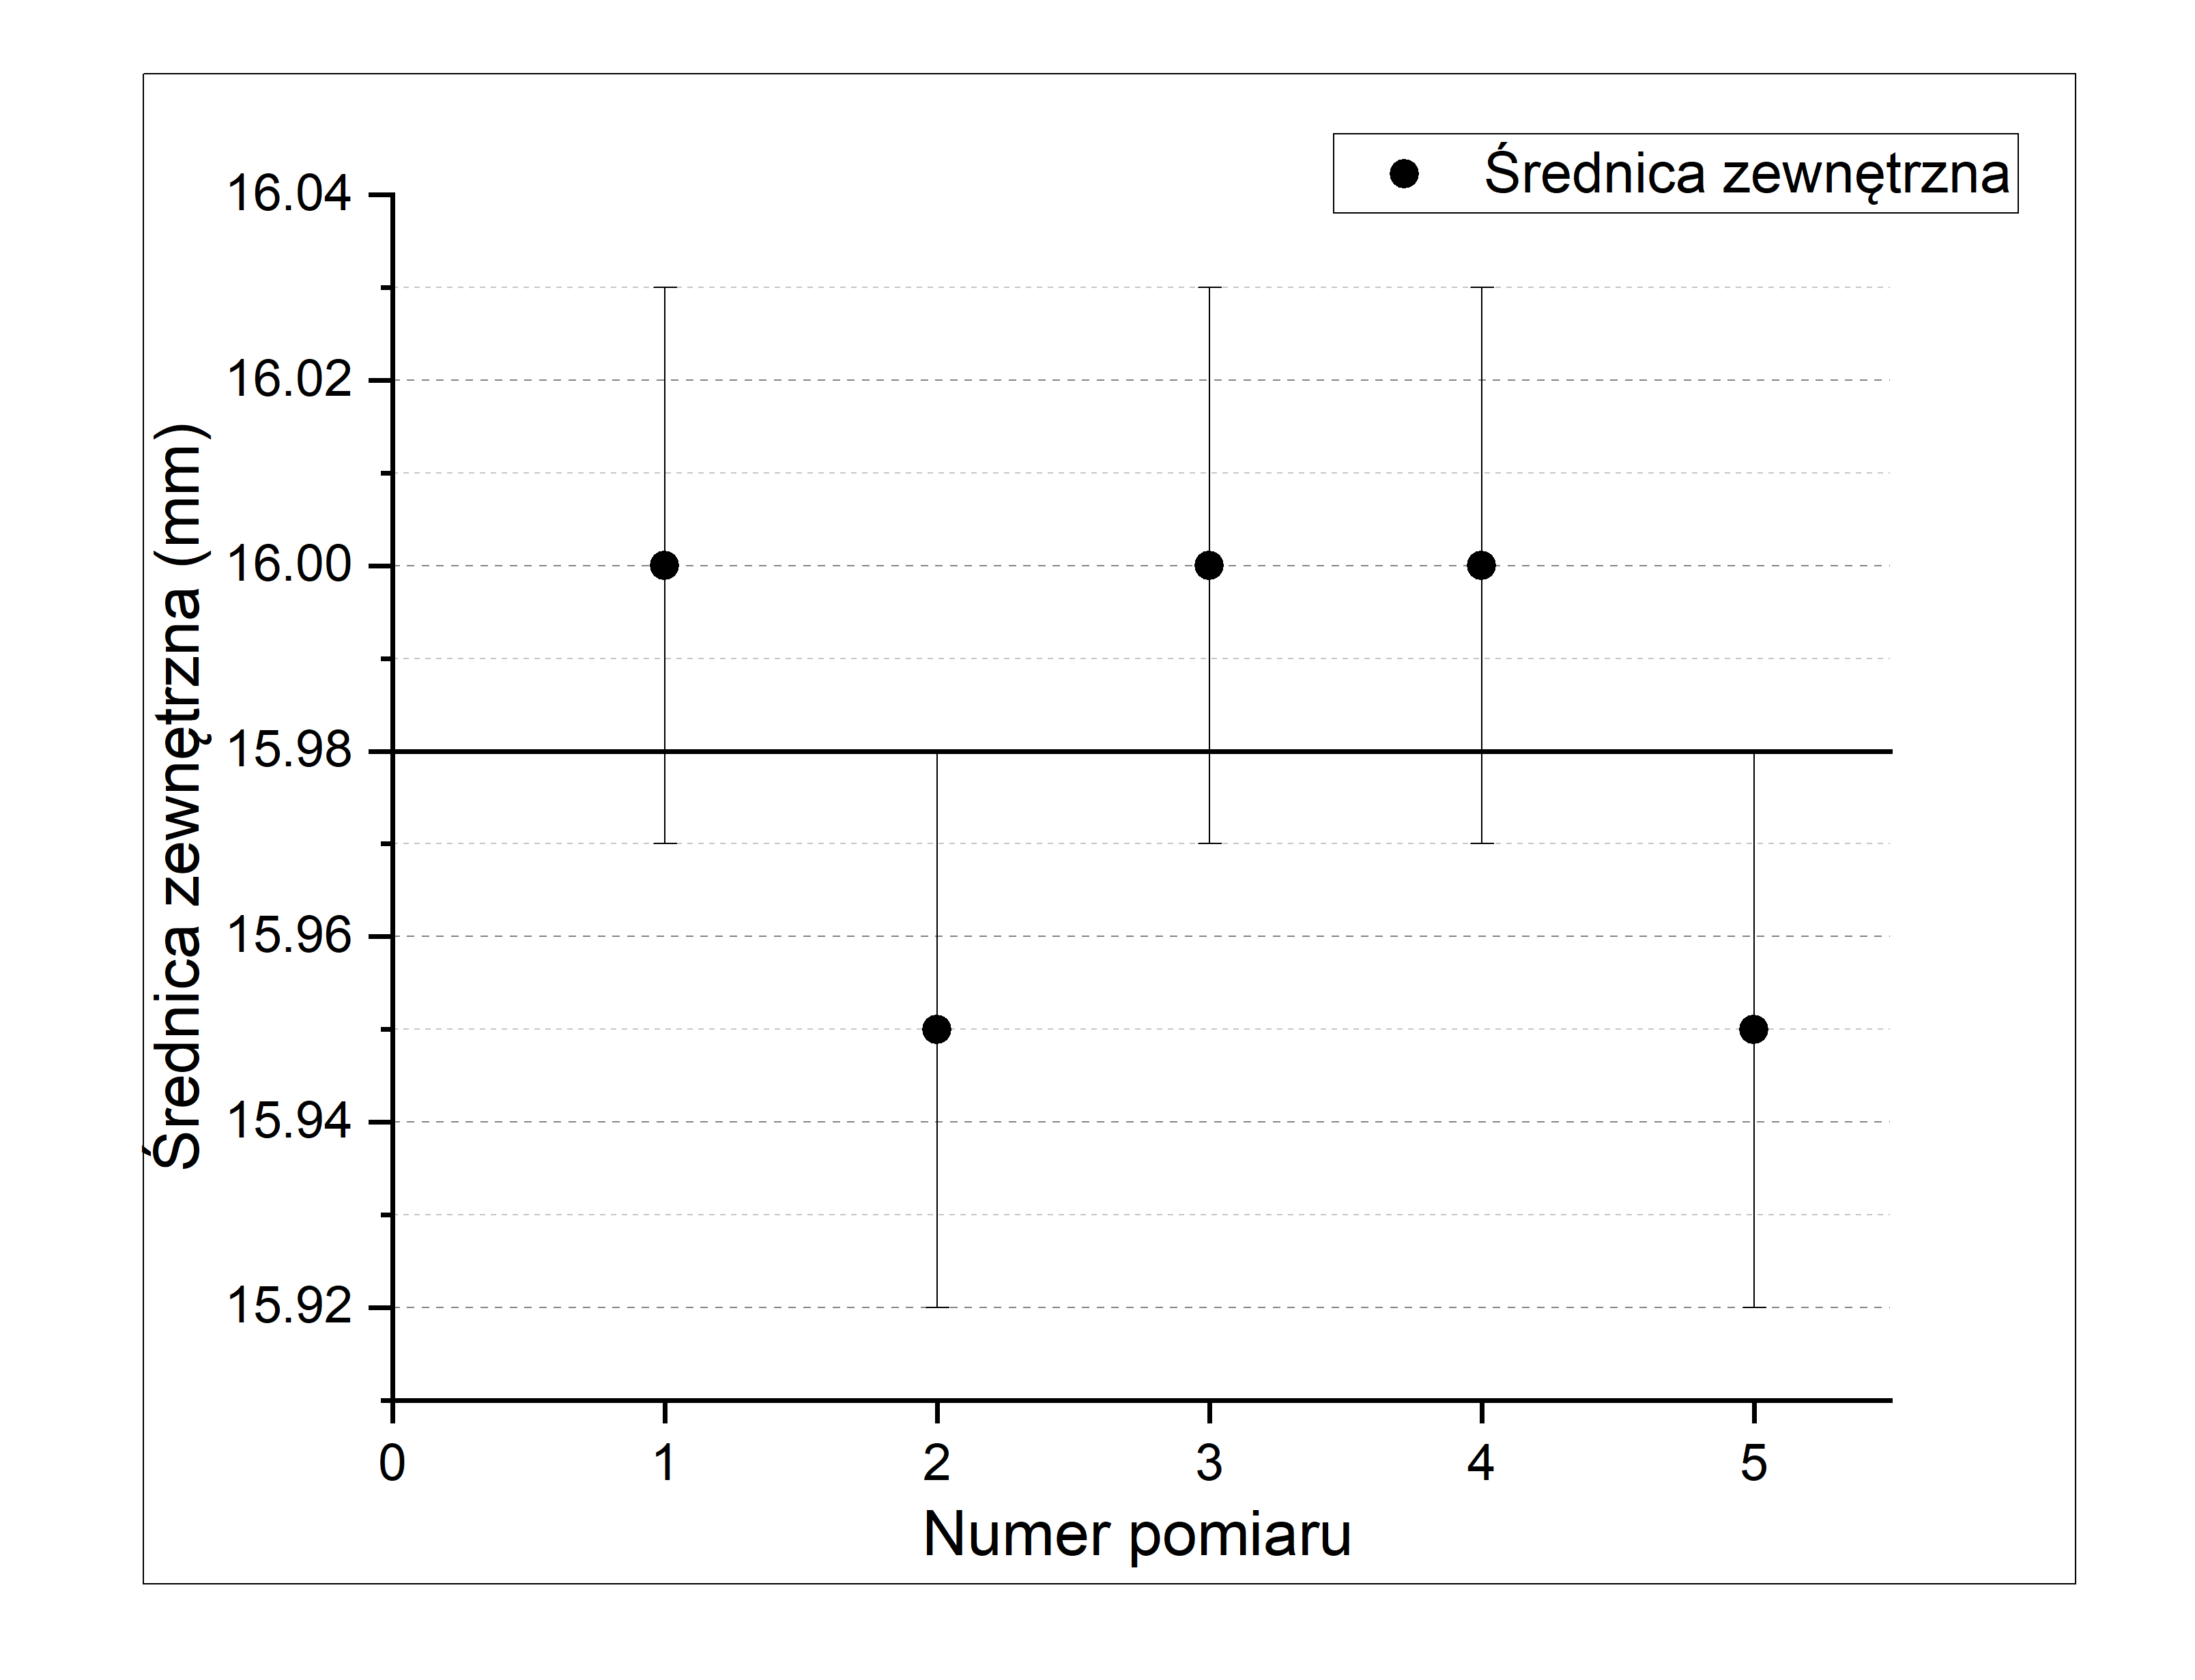
\includegraphics[width=70mm]{imgs/cylinder_2.png}
    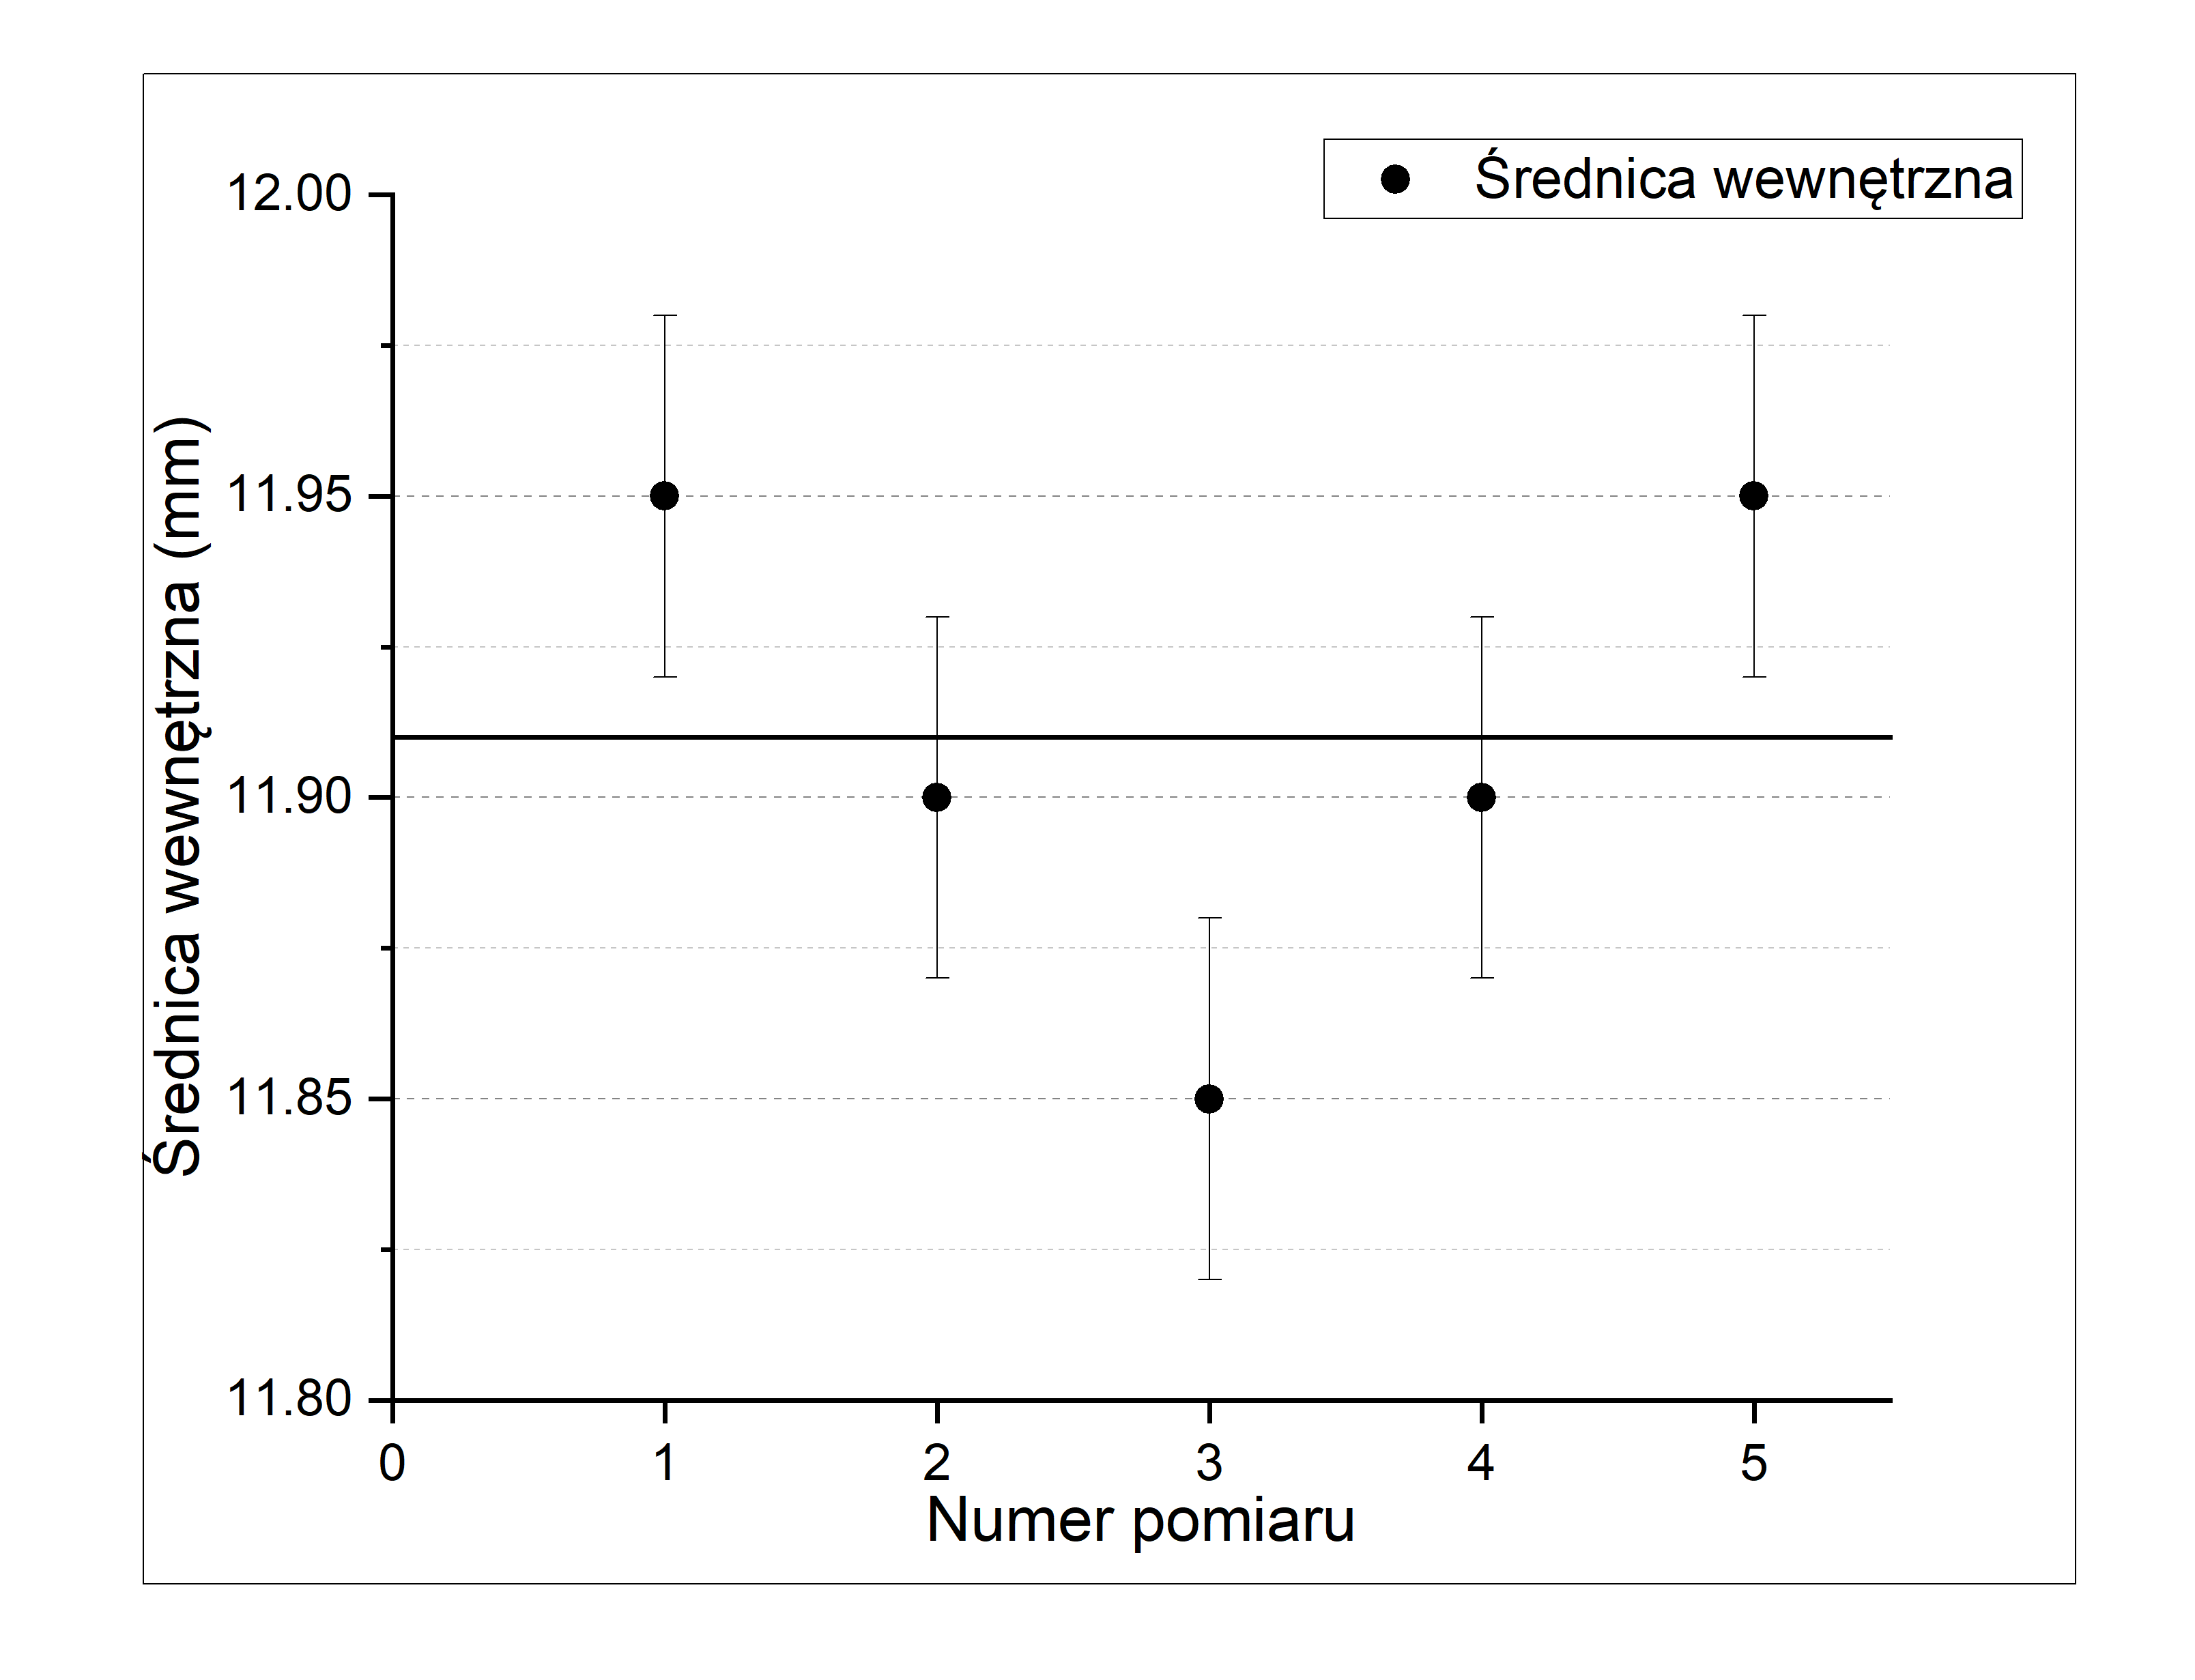
\includegraphics[width=70mm]{imgs/cylinder_1.png}
    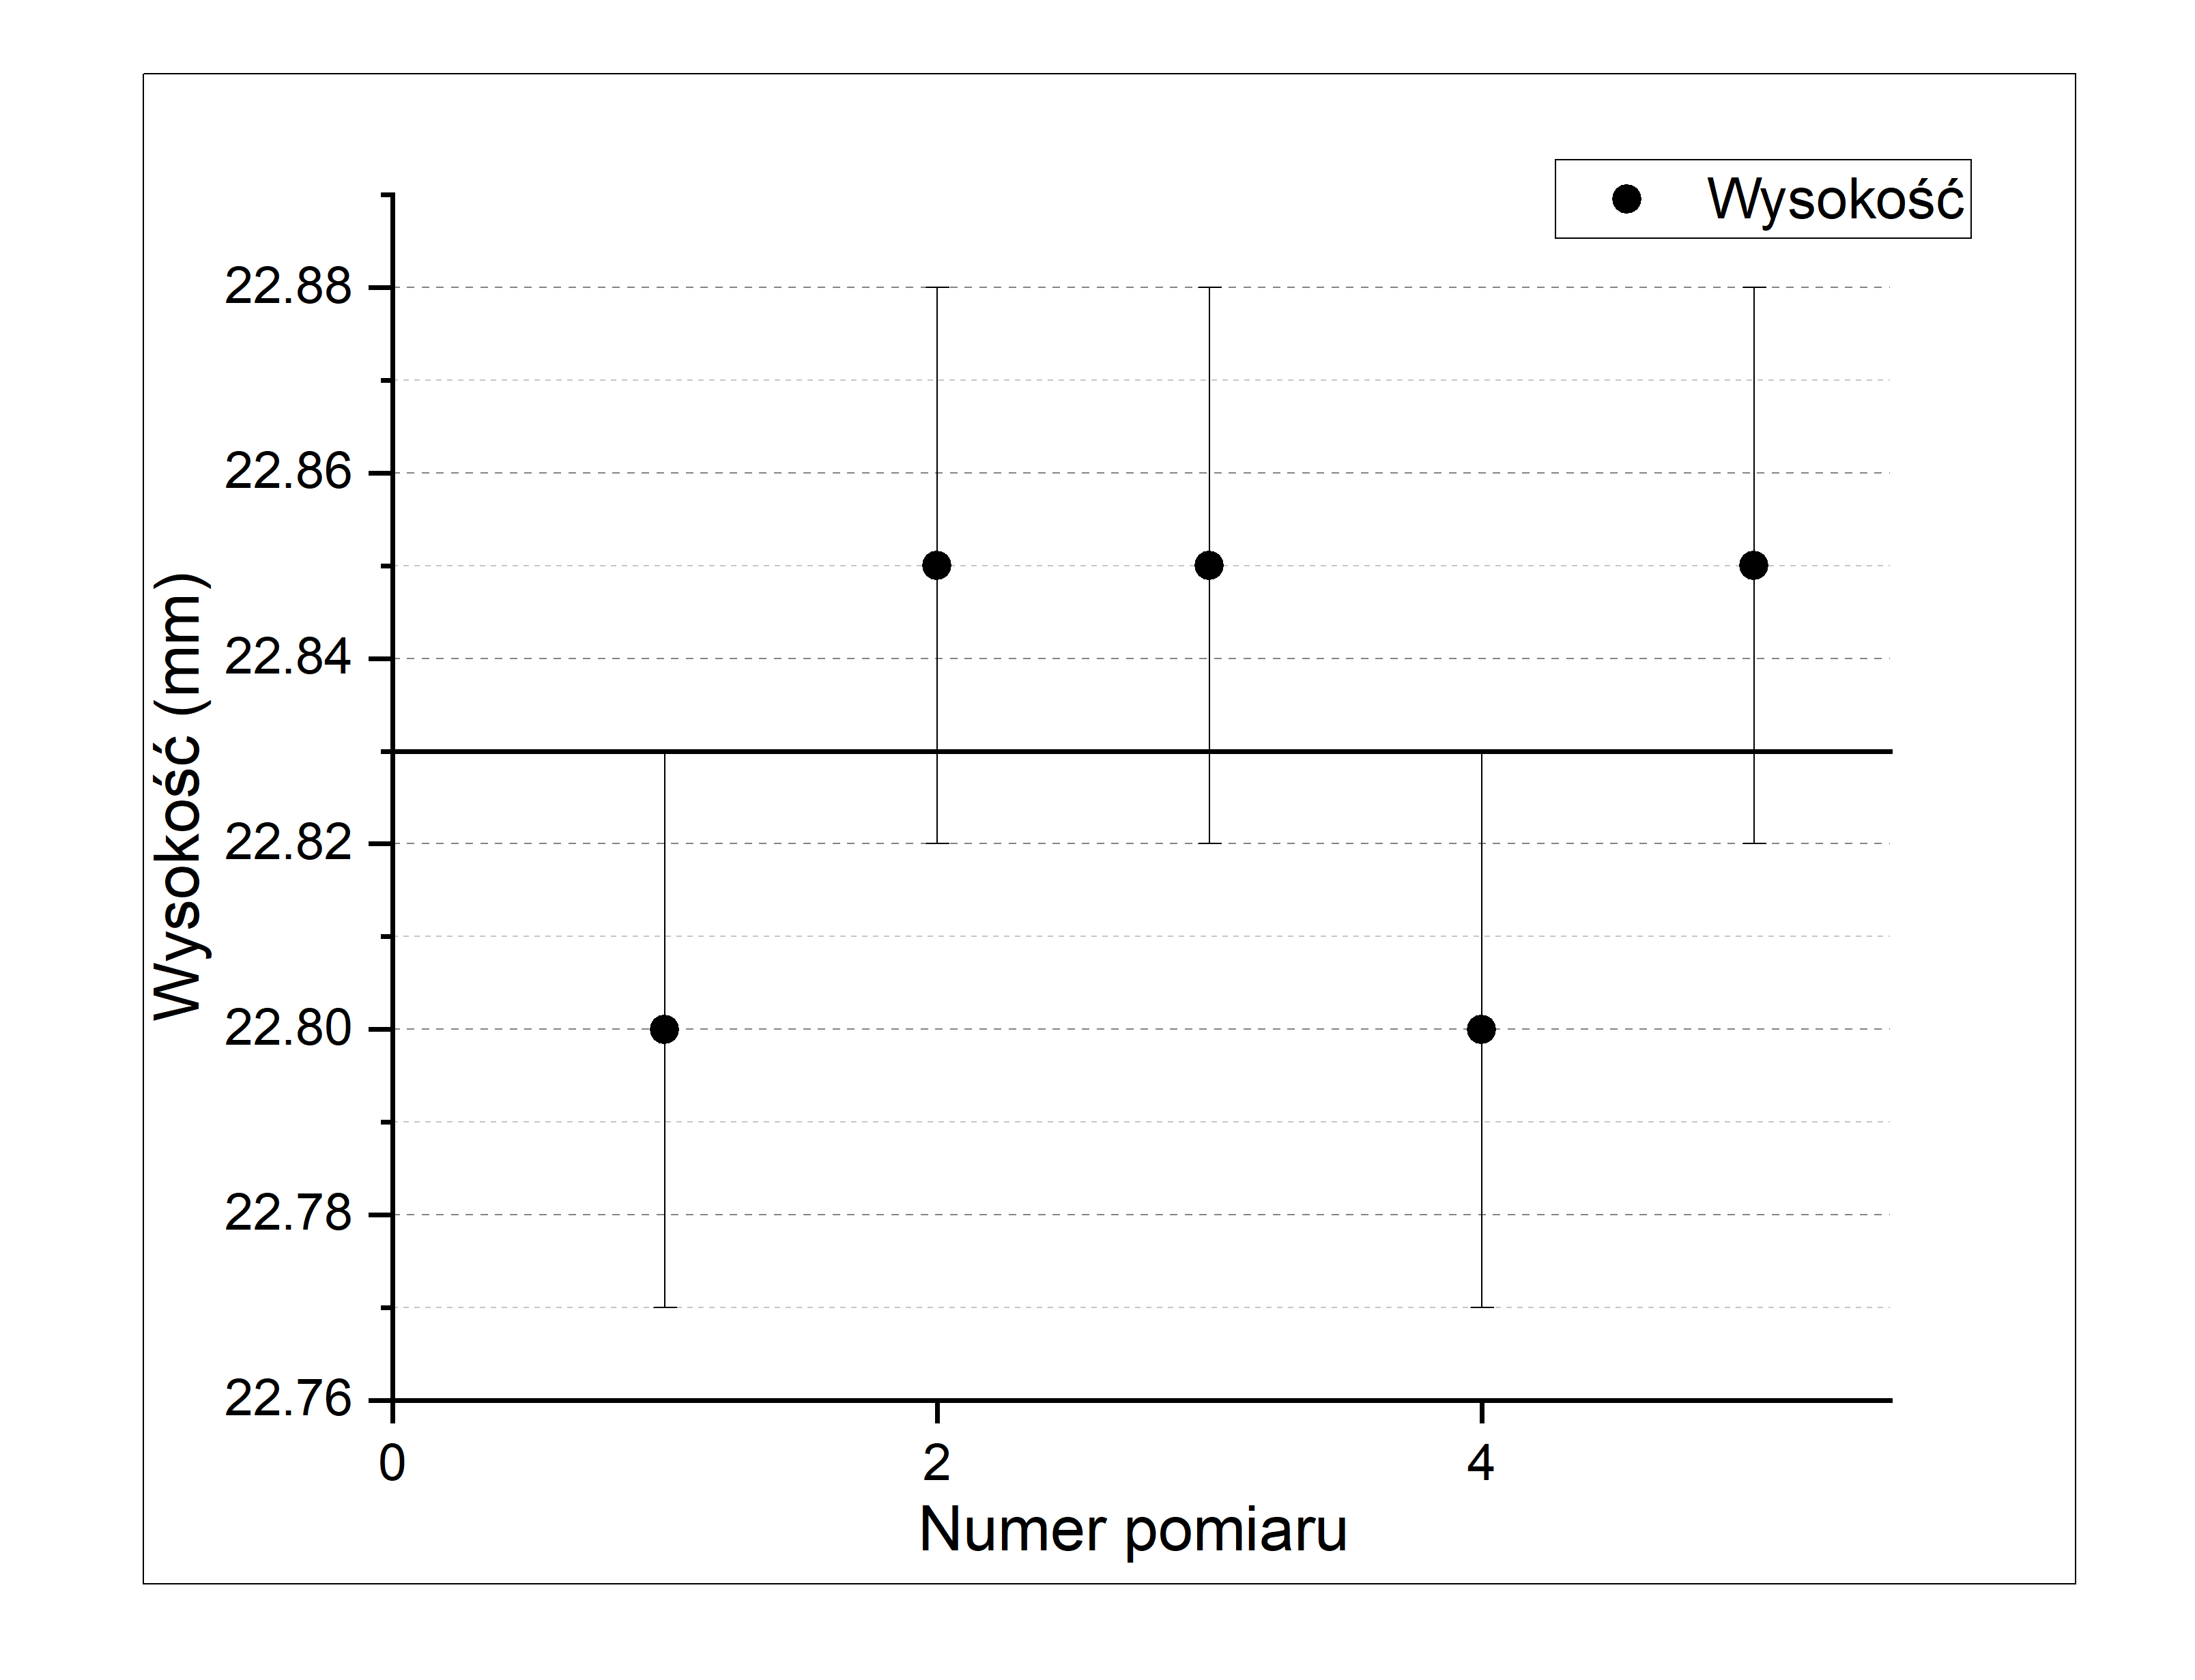
\includegraphics[width=70mm]{imgs/cylinder_3.png}
    \caption{Wyniki pomiarów cylindra.}
    \label{fig:cylinder_pomiary}
\end{figure}

{\subsection{Wałek}}

Tak samo jak w przypadku cylindra dla każdego wymiaru wykonano po 5 pomiarów.
Wymiary zmierzone w tym przypadku, to 6 średnic, 6 długości, oraz szerokość i długość frezu.
Wyniki pomiarów oraz obliczone niepewności ukazane są w tabelach poniżej: \\

{\indent \small \textit{Wszystkie wartości pomiarów podane są w $mm$.}}

\begin{center}
    \begin{tabular}{|r|c|c|c|c|c|c| |c|c|c|c|c|c|}
        \hline
        & \multicolumn{6}{|c||}{Średnice} & \multicolumn{6}{|c|}{Długości}\\
        \hline
        Lp.  & $\phi_1$ & $\phi_2$ & $\phi_3$ & $\phi_4$ & $\phi_5$ & $\phi_6$   & $d_1$ & $d_2$ & $d_3$ & $d_4$ & $d_5$ & $d_6$ \\
        \hline
        1.   & 10    & 14.95 & 21.65 & 18.1 & 21.65 & 14.2                       & 7  & 7.6 & 12.1  & 4.6  & 25.6  & 3.3  \\
        \hline
        2.   & 10.05 & 14.95 & 21.65 & 18.1 & 21.6  & 14.2                       & 7  & 7.6 & 12.1  & 4.55 & 25.65 & 3.35 \\
        \hline
        3.   & 10    & 14.95 & 21.65 & 18.1 & 21.65 & 14.2                       & 7  & 7.6 & 12.1  & 4.65 & 25.65 & 3.25 \\
        \hline
        4.   & 10.1  & 14.95 & 21.65 & 18.1 & 21.65 & 14.25                      & 7  & 7.6 & 12.15 & 4.6  & 25.6  & 3.3  \\
        \hline
        5.   & 10    & 14.95 & 21.65 & 18.1 & 21.65 & 14.2                       & 7  & 7.6 & 12.1  & 4.6  & 25.6  & 3.3  \\
        \hline
        $u_A(x)$ & 0.02 & 0 & 0 & 0 & 0.01 & 0.01                                & 0 & 0 & 0.01 & 0.0158 & 0.0122 & 0.0158\\
        \hline
        $u_B(x)$ & \multicolumn{12}{|c|}{0.03} \\
        \hline
        $u(x)$ & 0.04 & 0.03 & 0.03 & 0.03 & 0.03 & 0.03                         & 0.04 & 0.03 & 0.03 & 0.03 & 0.03 & 0.03\\
        \hline
    \end{tabular}

    \vspace{5mm}

    \begin{tabular}{|r|c|c|}
        \hline
        \multicolumn{3}{|c|}{Frez} \\
        \hline
        Lp.  & $s_f$ & $d_f$ \\
        \hline
        1.   & 12.9  & 9.6  \\
        \hline
        2.   & 12.95 & 9.55 \\
        \hline
        3.   & 12.9  & 9.6  \\
        \hline
        4.   & 12.9  & 9.6  \\
        \hline
        5.   & 12.9  & 9.55 \\
        \hline
        $u_A(x)$ & 0.01 & 0.0122 \\
        \hline
        $u_B(x)$ & \multicolumn{2}{|c|}{0.03} \\
        \hline
        $u(x)$ & 0.03 & 0.03 \\
        \hline
    \end{tabular}
\end{center}


